\section{Analisi statica}

\begin{frame}{Estrazione delle capabilities}
Dato un file eseguibile, andiamo a estrarre le \emph{capabilities}: quali azioni il programma è in grado di compiere

\vfill

\textbf{Come?} \\
Usiamo \emph{capa}, strumento open source realizzato da Mandiant

\vfill

\textbf{Perchè?} \\
Molto flessibile, con la possibilità di scrivere proprie regole custom in YAML
\end{frame}

\begin{frame}{Capabilities ottenute}
\begin{figure}
    \centering
    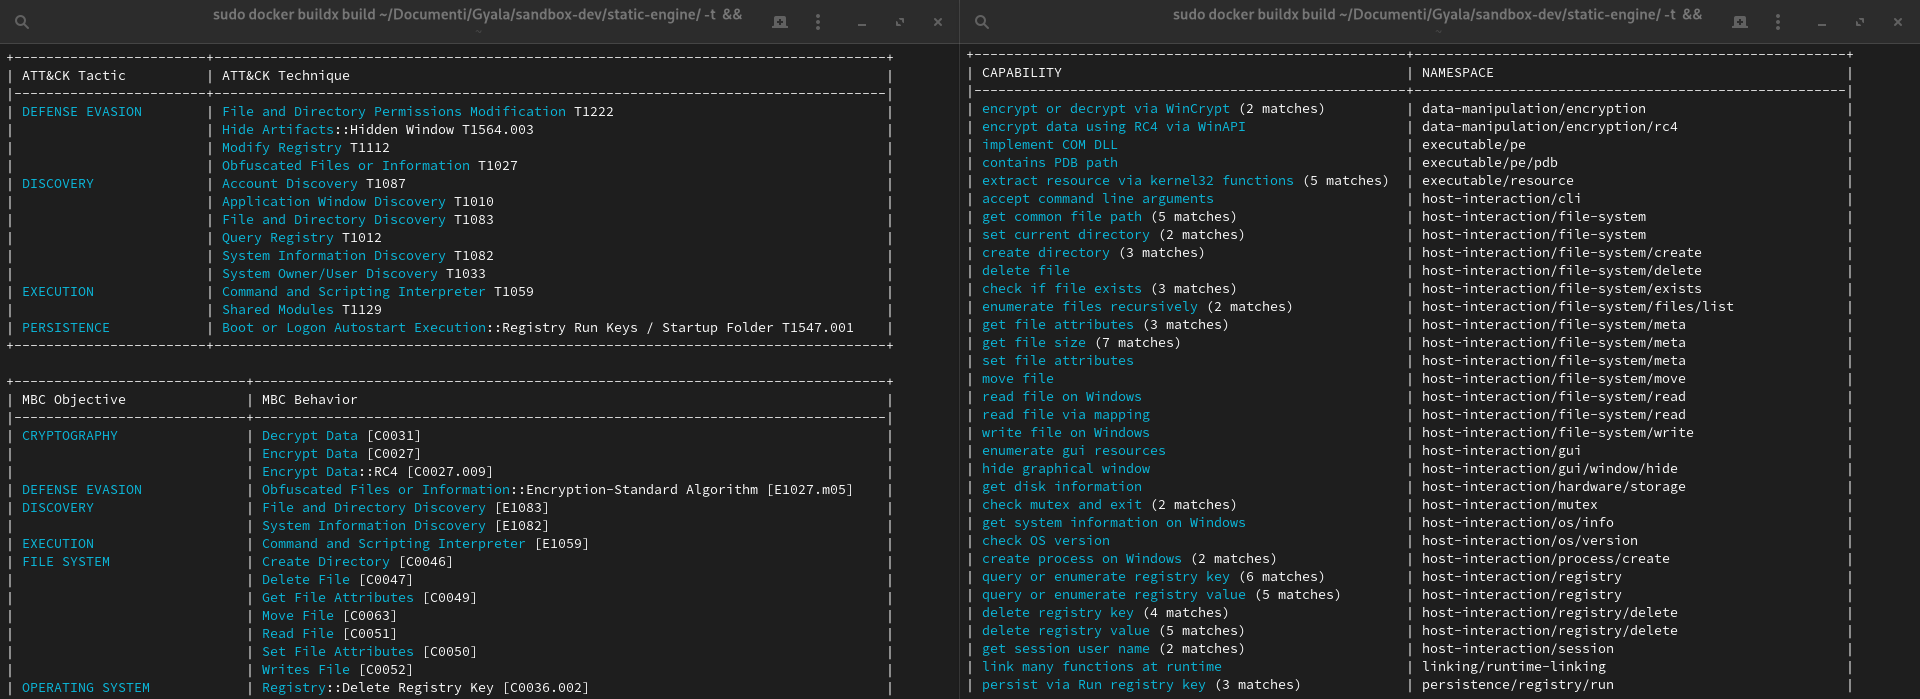
\includegraphics[width=\textwidth]{images/capa_example_invocation.png}
    \caption{Output restituito da capa}
    \label{fig:capa_example_invocation}
\end{figure}
\end{frame}

\begin{frame}{Parsing dell'output}
Non è un formato utilizzabile, bisogna farne il parsing.

\vfill

Notiamo la divisione in tabelle, e andiamo a trasformarlo in un JSON.

Lavoreremo sempre con formato JSON per essere sia human-readable dall'analista che machine-readable da servizi esterni.
\end{frame}

\begin{frame}{Output JSON}
\begin{figure}
    \centering
    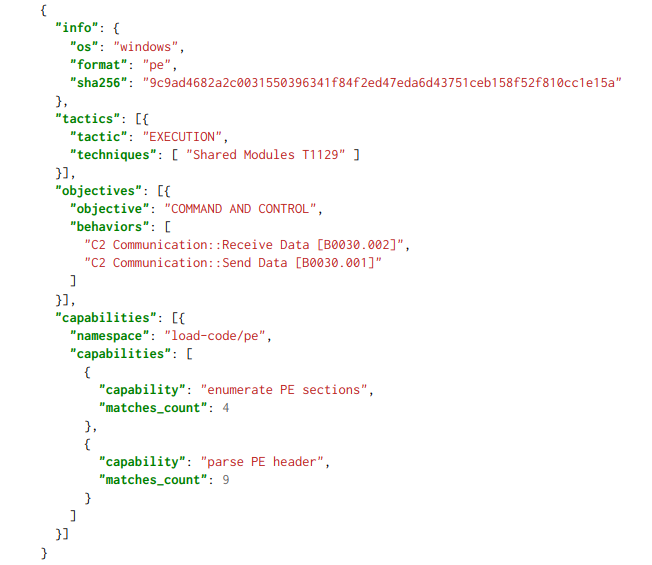
\includegraphics[width=0.57\textwidth]{images/capa_json_output.png}
    \caption{Output dopo il parsing}
    \label{fig:capa_json_output}
\end{figure}
\end{frame}

\begin{frame}{Casi non supportati}
Viene fatta analisi statica del codice per estrarre le capabilities.

Questo non funziona nei casi di eseguibile pacchettizzato, installer o con runtime particolari (es: Visual Basic).
\vfill
capa terminerà con \textbf{exit code 14}
\end{frame}

\begin{frame}{Conseguenze del crash}
\begin{itemize}
    \item Può portare a un fallimento dell'intero processo di analisi statica
    \item Crea spreco di risorse (CPU e memoria) per diversi minuti
\end{itemize}
\end{frame}

\begin{frame}{Rilevazione del caso non supportato}
Ci sono regole capa specifiche che rilevano questi casi, ma eseguirle richiede svariati minuti.

Dobbiamo creare un rilevatore custom da zero, basandoci sulle regole.

\begin{figure}
    \centering
    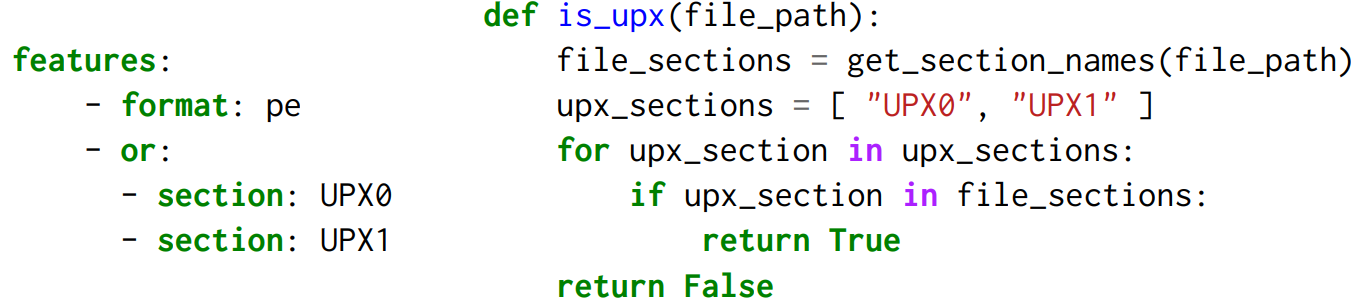
\includegraphics[width=\textwidth]{images/capa_detector_rule.png}
    \caption{Esempio di codice Python per simulare una regola}
    \label{fig:capa_detector_rule}
\end{figure}
\end{frame}

\begin{frame}{Struttura delle classi per il programma di rilevazione}
Le regole lavorano principalmente sul nome delle sezioni o presenza di stringhe.

\begin{figure}
    \centering
    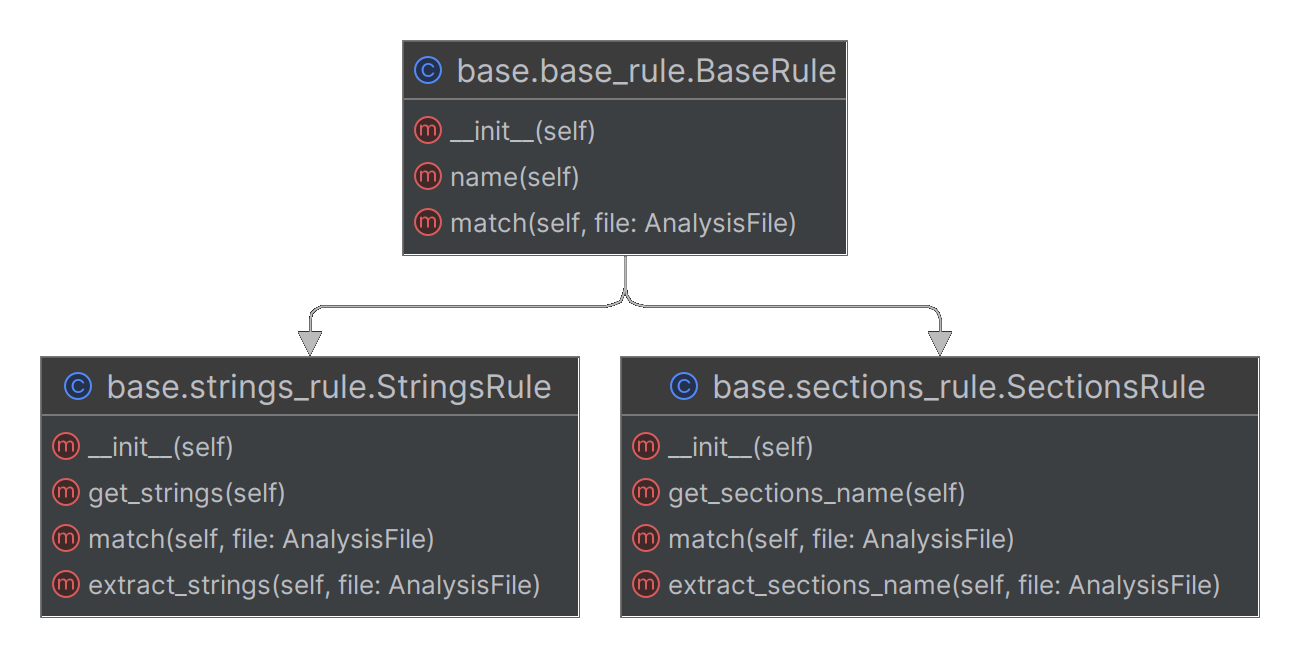
\includegraphics[width=0.7\textwidth]{images/base_custom_static_analyzer.png}
    \caption{Diagramma delle superclassi}
    \label{fig:base_custom_static_analyzer}
\end{figure}
\end{frame}

\begin{frame}{Velocità del rilevatore}
La rilevazione durerà meno di un secondo, a fronte di svariati minuti iniziali.

\begin{figure}
    \centering
    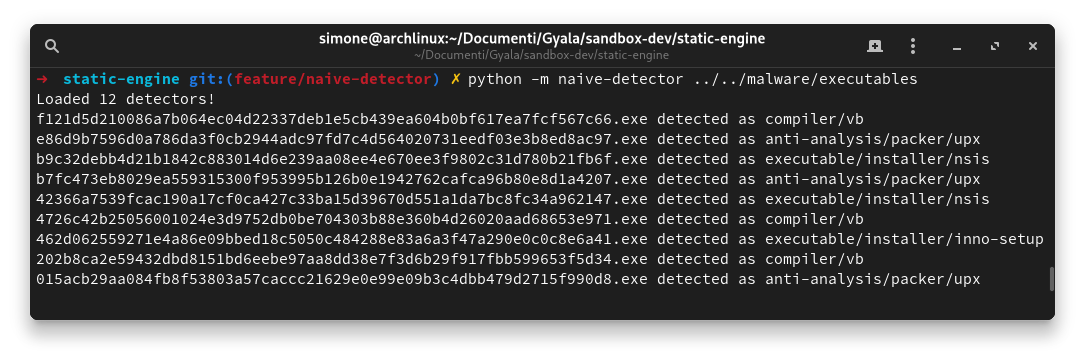
\includegraphics[width=\textwidth]{images/custom_file_detector_output.png}
    \caption{Esecuzione del rilevatore}
    \label{fig:custom_file_detector_output}
\end{figure}
\end{frame}

\begin{frame}{YARA}
Si esegue anche signature-based matching con lo strumento YARA.
\vfill
Colleziona regole da varie realtà della cybersecurity (aziende, ricercatori, ...) \\
oltre a tutte quelle sviluppate internamente
\vfill
Per ottimizzare l'esecuzione, le regole sono state divise in cartelle ed eseguite solo quando necessario, in base al sistema operativo target
\end{frame}

\begin{frame}{Ulteriori strumenti}
\begin{itemize}
    \item \textbf{SSDeep} per fuzzy hashing e correlazione di sample simili tra loro
    \item \textbf{Detect-It-Easy} e \textbf{ExifTool} estraggono ulteriori metadati dal file in analisi (linker utilizzato, descrizioni, charset, tabella dei simboli, ...)
\end{itemize}

\vfill

Tutti integrati in un \emph{unico flusso di esecuzione} e uniti in uno stesso risultato JSON finale, continuando ad eseguire parsing e trasformazioni di ciò che otteniamo dagli strumenti grezzi
\end{frame}

\begin{frame}{Flusso di esecuzione}
\begin{figure}
    \centering
    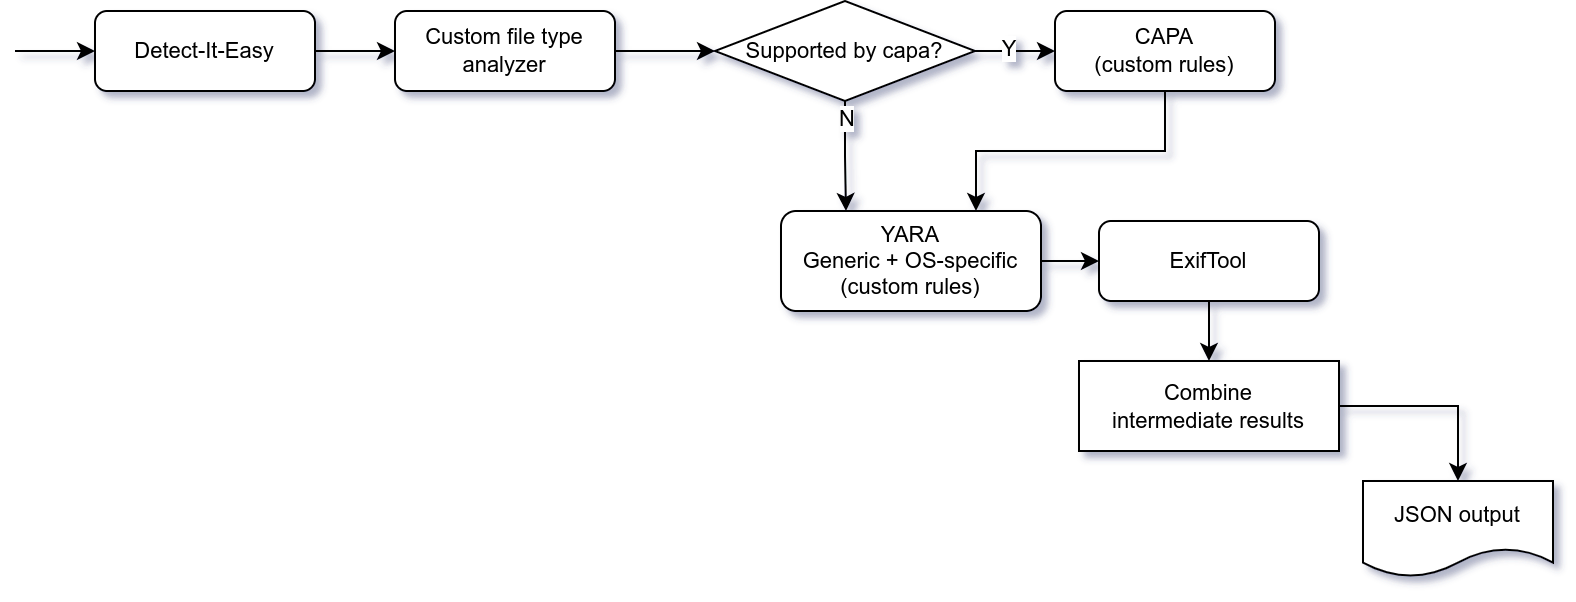
\includegraphics[width=0.9\textwidth]{images/static_run_analysis_internal_tools.png}
\end{figure}
La gestione degli errori avviene tramite handle degli exit-code e restituzione di un JSON contenente il campo \emph{"error"} con un error code tra le stringhe predeterminate
\end{frame}

\begin{frame}{Containerizzazione}
Viene incluso in un container Docker comprensivo di tutte le dipendenze, per massimizzare la portabilità.

Grazie all'uso intensivo di \textbf{multi-stage build} si è ridotta la sua dimensione finale a $\approx$ 200 MB, partendo da oltre 2 GB se creata in modo naive

Sfrutta anche la cache per le build seguenti e la parallelizzazione usando \texttt{docker buildx}
\end{frame}

\begin{frame}{Multi-stage build}

\begin{figure}
    \centering
    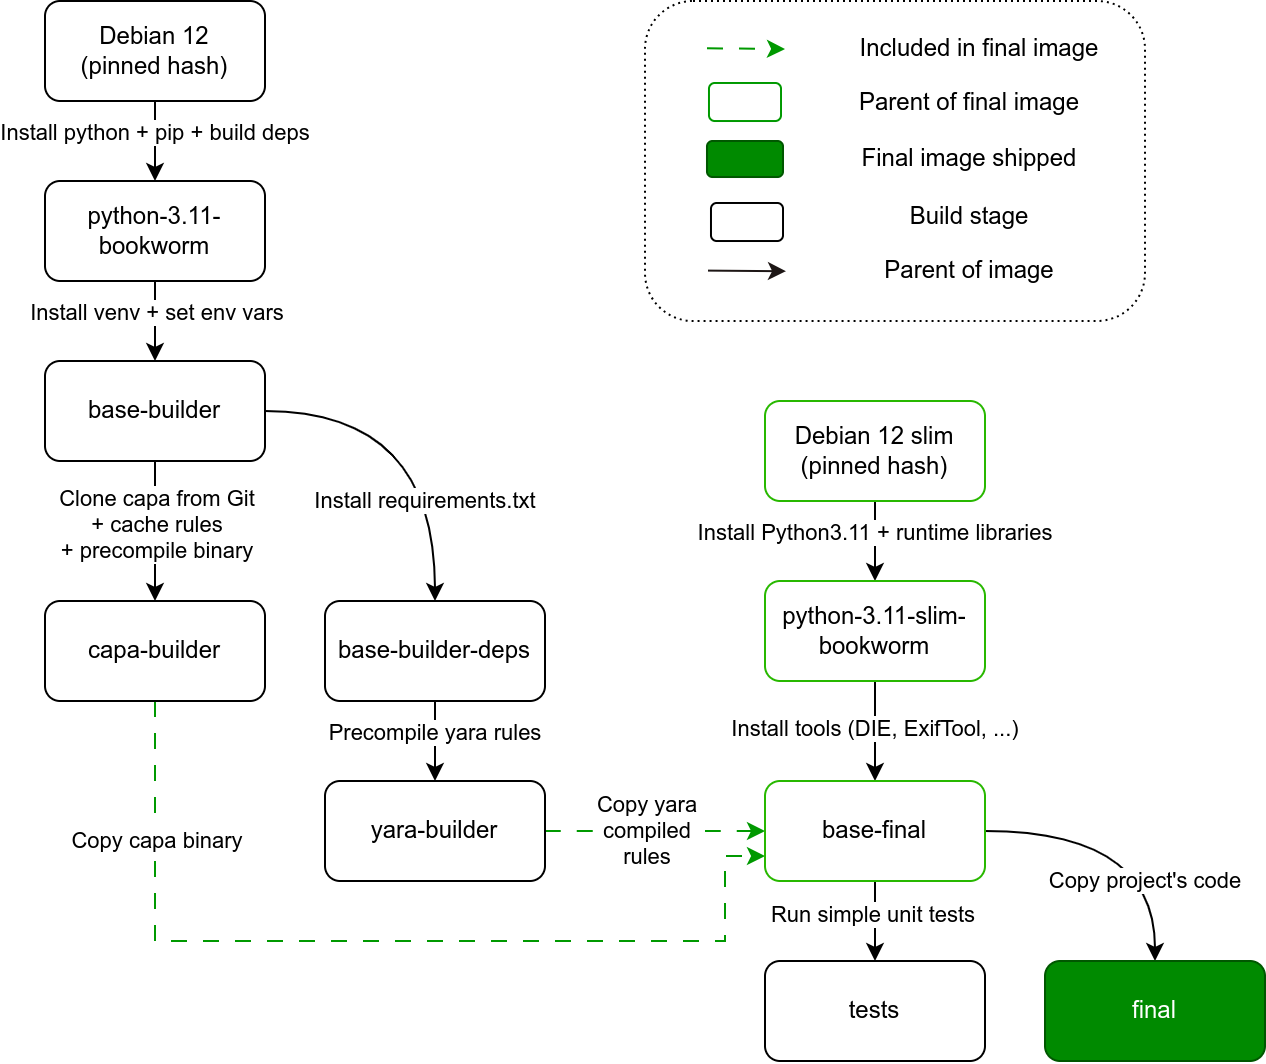
\includegraphics[width=0.6\textwidth]{images/dockerfile.png}
\end{figure}
\end{frame}

\begin{frame}{Deploy su AWS}
Dopo un'analisi dei costi e delle caratteristiche di AWS Lambda, EC2 e simili, si è optato per eseguire questa analisi su AWS Lambda.
\vfill
Si creano varie Lambda per minimizzare i permessi assegnati dove viene effettivamente analizzato il malware, seguendo il principio del \emph{Least Privilege}
\end{frame}

\begin{frame}{Architettura AWS}
\begin{figure}
    \centering
    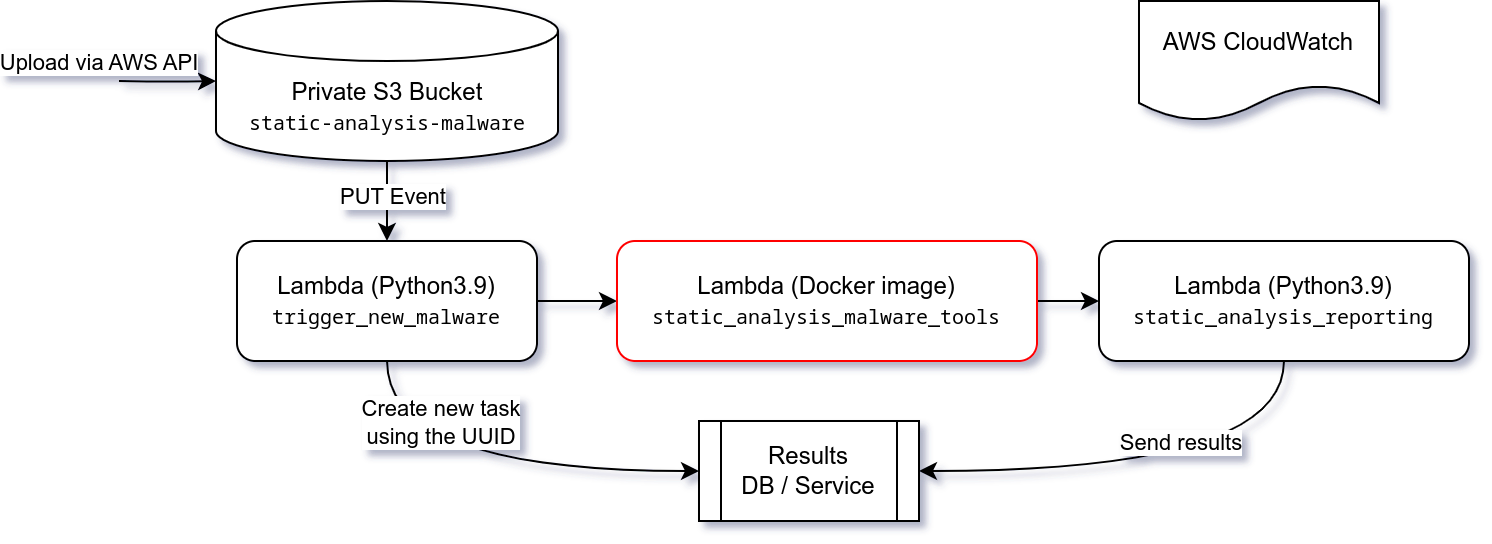
\includegraphics[width=\textwidth]{images/aws_static_lambdas_architecture.png}
\end{figure}
\end{frame}

\begin{frame}{Compressione del risultato}
Per non usare inutilmente un bucket S3 per salvare i risultati, viene passato il JSON finale da \texttt{static\_analysis\_malware\_tools} a \texttt{static\_analysis\_reporting}.
\vfill
AWS limita questo payload a 6MB, spesso viene superato.
\vfill
Si è scelto di comprimere il JSON con gzip, poi reso una stringa ASCII usando Base64.
Se ancora si superano i 6MB si emette un errore, ma è un caso raro o dovuto a regole YARA mal scritte.
\end{frame}

\begin{frame}{Compressione del risultato}
\begin{figure}
    \centering
    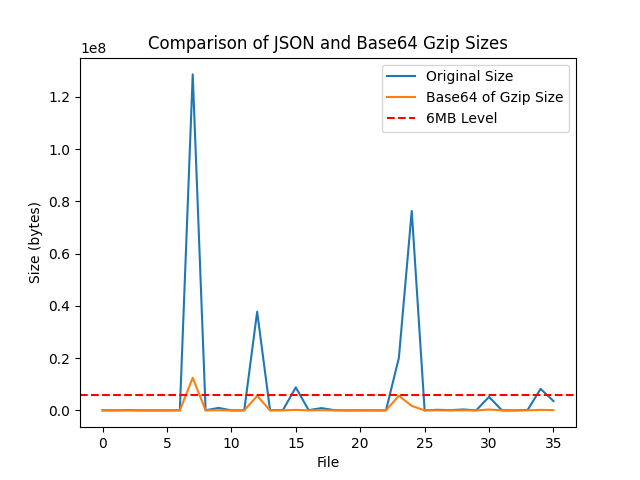
\includegraphics[width=0.5\textwidth]{images/static_analysis_results_size.png}
    \caption{Differenza tra la dimensione prima e dopo la compressione}
    \label{fig:static_analysis_results_size}
\end{figure}
\end{frame}

\begin{frame}{Pipeline CI/CD}
Per automatizzare anche il processo di deploy dello strumento, si è creata una pipeline CI/CD su GitLab che esegue in appositi Runner.
\vfill
Così, se si modifica una regola o esegue una modifica, al push del commit Git viene eseguito:
\begin{itemize}
    \item \textbf{build} dell'immagine Docker
    \item \textbf{test} usando dei file innocui creati per varie architetture, sistemi operativi e casistiche (tradizionali, packed, installer, ...)
    \item \textbf{deploy} dell'immagine su AWS ECR e sulla Lambda in caso di test positivi
\end{itemize}
\end{frame}